\scalebox{1}{
    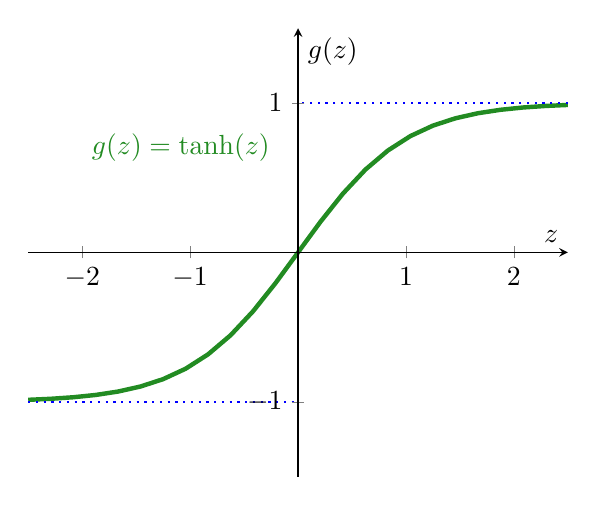
\begin{tikzpicture}
        \begin{axis}[
            xmin=-2.5, xmax=2.5,
            ymin=-1.5, ymax=1.5,
            axis lines=center,
            axis on top=true,
            domain=-2.5:2.5,
            ylabel=$g(z)$,
            xlabel=$z$,
            ]
        
            \addplot [mark=none,draw=ForestGreen,ultra thick] {tanh(\x)};
            \node [right, ForestGreen] at (axis cs: -2,0.7) {$g(z) = \tanh (z)$};
            
            %% Add the asymptotes
            \draw [blue, dotted, thick] (axis cs:-2.5,-1)-- (axis cs:0,-1);
            \draw [blue, dotted, thick] (axis cs:+2.5,+1)-- (axis cs:0,+1);
        \end{axis}
    \end{tikzpicture}
}